\documentclass[onlytextwidth]{beamer}
\documentclass[onlytextwidth]{beamer}
\usepackage[utf8]{inputenc}
\usepackage{microtype}
\usepackage{amsmath}
\usepackage{amssymb}
\usepackage[nomessages]{fp} %\FPeval{\var-name}{2*sin(pi/6)}
\usepackage{siunitx} %units in math. eg 20\milli\meter
\usepackage{yhmath} % for arcs, overparenth command
\usepackage{tikz} %graphics
\usetikzlibrary{quotes, angles}
%\usepackage{graphicx} already loaded by beamer class
%consider setting \graphicspath{{images/}}
%\parskip ?? to avoid paragraph indent
\usepackage{multicol} %may not need this package, just columns environment
\usepackage{venndiagram}

\subtitle[BECA]{Bronx Early College Academy}
\author[Huson]{Christopher J. Huson PhD}

\setbeamertemplate{headline}{\vskip2mm 
  BECA / \insertshortauthor \, / \inserttitle
  \hfill 
  \insertsection
  }

\title{Routines and Expectations}
\date{2023-2024}

\begin{document}
\frame{\titlepage}

%\section[Outline]{}
%\frame{\tableofcontents}

\section{0.1 Personal tools every day \hfill 7 September}
\begin{frame}{Begin class on time}
  {Sign in when late \hfill \alert{0.1 Thursday 7 September}}
  \begin{block}{Expectation: On your desk, every day, start of class}
  \begin{enumerate}
      \item Notebook, pencil/pen
      \item Pocket folder, lined paper (no spiral notebooks)
      \item Tools: calculator, laptop computer (charged)
  \end{enumerate}
  \end{block}
  Supply list: Composition book, folder, looseleaf, pencils \& pens, \\*
  ruler, calculator
  \end{frame}

\begin{frame}{Take class notes in a composition book}
  \begin{block}{Use this notebook format (required)}
    \begin{enumerate}
      \item Outside cover: ``Math'', your first and last name
      \item First page: your name, my contact info, your passwords \\
      \qquad Dr. Huson / chuson@schools.nyc.gov / 917-648-5632 \vspace{0.25cm}
      \item Each page in the top left corner: \\
      \emph{I can measure and estimate} \hfill 7 September 2023 \vspace{0.25cm}
      \item Copy definitions using your own words
      \item Write down example diagrams and problems
    \end{enumerate}
    \end{block}
  \end{frame}

\section{0.2 Casio calculator \hfill 7 September}
\begin{frame}{Casio fx-9750GIII calculator (due Friday 15 September)}
  \begin{columns}
    \column{0.4\textwidth}
      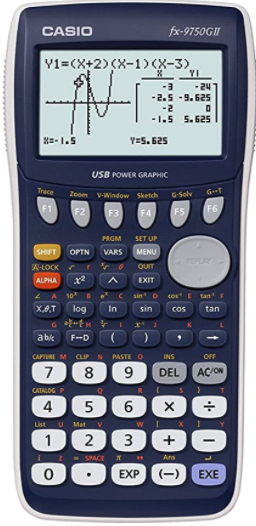
\includegraphics[width=2.75cm]{../graphics/casio_fx-9750GII.png}
    \column{0.6\textwidth}
      In the high school at BECA we use the Casio fx-9750GIII.\\[5pt] 
      It is allowed on the Regents exams, SAT tests, and International Baccalaureate exams.\\[5pt]
      The older model is also acceptable, Casio fx-9750\alert{GII}.\\[5pt]
      (see me if buying a calculator is a hardship for your family)
    \end{columns} \vspace{1cm}
  Supply list: Composition book, folder, looseleaf paper, pencils \& pens, ruler, calculator
\end{frame}

\section{0.3 Dismissal \hfill 7 September}
\begin{frame}{Follow routines to increase efficiency and reduce stress}
  \begin{block}{Write name on work immediately}
    \begin{enumerate}
      \item First and last name in upper right corner
    \end{enumerate}
    \end{block}
  \begin{block}{Bathroom / breaks are limited}
    \begin{enumerate}
      \item Request breaks only during allocated time
      \item Do not interrupt instruction
    \end{enumerate}
    \end{block}
  \begin{block}{Work until told to begin dismissal routine (3 minutes)}
    \begin{enumerate}
      \item Stay seated and quiet until dismissed
      \item Straighten desks, check for garbage, push in your chair
    \end{enumerate}
    \end{block}
  \end{frame}

\section{0.4 Laptop computers \hfill 7 September}
\begin{frame}{Computers are your responsibility}
  \begin{block}{Use only for school work}
    \begin{enumerate}
      \item Playing games or surfing is \emph{off task} and earns a poor participation grade
      \item ``Lids down'' when the teacher or a student is presenting
      \item Charge at home each night\\
        (4:75\%, 3: 50+\%, 2:20+\%, 1:0+, 0:dead)
      \item BECA computers are not private (GoGuardian)
    \end{enumerate}
    \end{block}
  \end{frame}

\section{Be your best}
\begin{frame}{Upper classmen have privileges and responsibilities}
  \begin{block}{I expect a lot from you}
    \begin{itemize}
      \item You are role models for the younger students
      \item These last high school years can be fun, but also...
      \item There is a lot of serious work this year
    \end{itemize}
    \end{block}
  \end{frame}

\section{Student quote}
\begin{frame}{You are not in middle school}
  \begin{block}{Advice from one of my students for kids coming next year}\vspace{0.5cm}
    ``Though your teaching skills are unique it just takes time to get used to. At the end you will realize that it is very helpful in the way that he teaches. You may not like it but you will grow to understand it. Stay in your seat and listen to Dr. Huson and raise your hand and ask questions.''
  \end{block}
  \end{frame}

\end{document}